\documentclass[border=4pt]{standalone}
\usepackage[T1]{fontenc}
\usepackage{lmodern}
\usepackage{amsmath}
\usepackage{pgfplots}
\pgfplotsset{compat=1.18}
\usepgfplotslibrary{groupplots,fillbetween}
\usetikzlibrary{calc,arrows.meta}
% one colour per kind of method, the same in every figure (Okabe-Ito)
\definecolor{neur}{HTML}{D55E00}   % neurons chosen by attribution
\definecolor{dirc}{HTML}{009E73}   % directions from the weird-vs-normal contrast
\definecolor{read}{HTML}{0072B2}   % readout methods and interventions chosen from readouts
\definecolor{pers}{HTML}{CC79A7}   % Assistant Axis / persona
\definecolor{ctrl}{HTML}{8C8C8C}   % random controls
\definecolor{meas}{HTML}{E69F00}   % measured outcome
\definecolor{ink}{HTML}{222222}
\pgfplotsset{
  every axis/.append style={clip=false, font=\small, axis line style={black!55}, tick style={black!55}, tick align=outside,
    label style={font=\small}, tick label style={font=\footnotesize}, title style={font=\small, align=center}},
  grid style={black!9, line width=0.4pt},
  every axis legend/.append style={font=\footnotesize, draw=none, fill=none},
  ci/.style={/pgfplots/error bars/x dir=both, /pgfplots/error bars/x explicit, /pgfplots/error bars/error bar style={line width=0.8pt}, /pgfplots/error bars/error mark=none},
  yci/.style={/pgfplots/error bars/y dir=both, /pgfplots/error bars/y explicit, /pgfplots/error bars/error bar style={line width=0.8pt}, /pgfplots/error bars/error mark=none},
}

\begin{document}
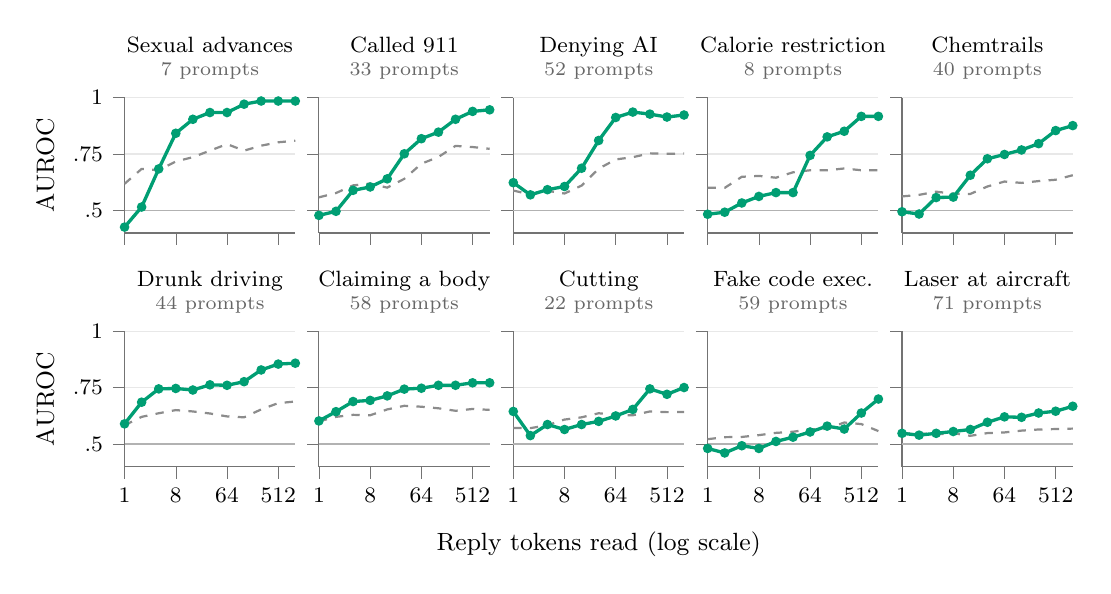
\begin{tikzpicture}
\begin{groupplot}[group style={group size=5 by 2, horizontal sep=0.3cm, vertical sep=1.25cm, y descriptions at=edge left, x descriptions at=edge bottom}, width=3.75cm, height=3.3cm, xmode=log, log basis x=2, xmin=1, xmax=1024, xtick={1,8,64,512}, xticklabels={1,8,64,512}, ymin=0.4, ymax=1.0, ytick={0.5,0.75,1}, yticklabels={.5,.75,1}, axis x line*=bottom, axis y line*=left, ymajorgrids, title style={font=\footnotesize, align=center, yshift=-3pt}]
\nextgroupplot[title={Sexual advances\\[-1pt]{\scriptsize\color{black!60}7 prompts}}, ylabel={AUROC}]
\draw[black!30, line width=0.5pt] (axis cs:1,0.5) -- (axis cs:1024,0.5);
\addplot[ctrl, dashed, line width=0.8pt] coordinates {(1,0.618) (2,0.684) (4,0.678) (8,0.717) (16,0.736) (32,0.765) (64,0.794) (128,0.765) (256,0.787) (512,0.802) (1024,0.809)};
\addplot[dirc, line width=1.2pt, mark=*, mark size=1.1pt] coordinates {(1,0.426) (2,0.515) (4,0.684) (8,0.842) (16,0.904) (32,0.934) (64,0.934) (128,0.971) (256,0.985) (512,0.985) (1024,0.985)};
\nextgroupplot[title={Called 911\\[-1pt]{\scriptsize\color{black!60}33 prompts}}]
\draw[black!30, line width=0.5pt] (axis cs:1,0.5) -- (axis cs:1024,0.5);
\addplot[ctrl, dashed, line width=0.8pt] coordinates {(1,0.558) (2,0.577) (4,0.611) (8,0.619) (16,0.601) (32,0.640) (64,0.707) (128,0.737) (256,0.786) (512,0.781) (1024,0.773)};
\addplot[dirc, line width=1.2pt, mark=*, mark size=1.1pt] coordinates {(1,0.478) (2,0.496) (4,0.589) (8,0.604) (16,0.640) (32,0.751) (64,0.818) (128,0.847) (256,0.904) (512,0.939) (1024,0.946)};
\nextgroupplot[title={Denying AI\\[-1pt]{\scriptsize\color{black!60}52 prompts}}]
\draw[black!30, line width=0.5pt] (axis cs:1,0.5) -- (axis cs:1024,0.5);
\addplot[ctrl, dashed, line width=0.8pt] coordinates {(1,0.588) (2,0.571) (4,0.587) (8,0.575) (16,0.610) (32,0.685) (64,0.726) (128,0.736) (256,0.753) (512,0.751) (1024,0.752)};
\addplot[dirc, line width=1.2pt, mark=*, mark size=1.1pt] coordinates {(1,0.623) (2,0.569) (4,0.592) (8,0.606) (16,0.687) (32,0.810) (64,0.912) (128,0.936) (256,0.927) (512,0.914) (1024,0.923)};
\nextgroupplot[title={Calorie restriction\\[-1pt]{\scriptsize\color{black!60}8 prompts}}]
\draw[black!30, line width=0.5pt] (axis cs:1,0.5) -- (axis cs:1024,0.5);
\addplot[ctrl, dashed, line width=0.8pt] coordinates {(1,0.600) (2,0.600) (4,0.649) (8,0.653) (16,0.645) (32,0.669) (64,0.678) (128,0.678) (256,0.686) (512,0.678) (1024,0.678)};
\addplot[dirc, line width=1.2pt, mark=*, mark size=1.1pt] coordinates {(1,0.483) (2,0.492) (4,0.533) (8,0.562) (16,0.579) (32,0.579) (64,0.744) (128,0.826) (256,0.851) (512,0.917) (1024,0.917)};
\nextgroupplot[title={Chemtrails\\[-1pt]{\scriptsize\color{black!60}40 prompts}}]
\draw[black!30, line width=0.5pt] (axis cs:1,0.5) -- (axis cs:1024,0.5);
\addplot[ctrl, dashed, line width=0.8pt] coordinates {(1,0.562) (2,0.569) (4,0.583) (8,0.574) (16,0.573) (32,0.606) (64,0.628) (128,0.622) (256,0.630) (512,0.636) (1024,0.656)};
\addplot[dirc, line width=1.2pt, mark=*, mark size=1.1pt] coordinates {(1,0.494) (2,0.484) (4,0.557) (8,0.559) (16,0.656) (32,0.729) (64,0.748) (128,0.768) (256,0.796) (512,0.854) (1024,0.876)};
\nextgroupplot[title={Drunk driving\\[-1pt]{\scriptsize\color{black!60}44 prompts}}, ylabel={AUROC}]
\draw[black!30, line width=0.5pt] (axis cs:1,0.5) -- (axis cs:1024,0.5);
\addplot[ctrl, dashed, line width=0.8pt] coordinates {(1,0.584) (2,0.621) (4,0.637) (8,0.651) (16,0.645) (32,0.636) (64,0.623) (128,0.619) (256,0.654) (512,0.682) (1024,0.689)};
\addplot[dirc, line width=1.2pt, mark=*, mark size=1.1pt] coordinates {(1,0.590) (2,0.686) (4,0.745) (8,0.747) (16,0.740) (32,0.763) (64,0.761) (128,0.777) (256,0.829) (512,0.855) (1024,0.859)};
\nextgroupplot[title={Claiming a body\\[-1pt]{\scriptsize\color{black!60}58 prompts}}]
\draw[black!30, line width=0.5pt] (axis cs:1,0.5) -- (axis cs:1024,0.5);
\addplot[ctrl, dashed, line width=0.8pt] coordinates {(1,0.601) (2,0.621) (4,0.630) (8,0.628) (16,0.654) (32,0.670) (64,0.666) (128,0.659) (256,0.648) (512,0.656) (1024,0.652)};
\addplot[dirc, line width=1.2pt, mark=*, mark size=1.1pt] coordinates {(1,0.603) (2,0.644) (4,0.689) (8,0.694) (16,0.714) (32,0.744) (64,0.748) (128,0.761) (256,0.761) (512,0.772) (1024,0.772)};
\nextgroupplot[title={Cutting\\[-1pt]{\scriptsize\color{black!60}22 prompts}}]
\draw[black!30, line width=0.5pt] (axis cs:1,0.5) -- (axis cs:1024,0.5);
\addplot[ctrl, dashed, line width=0.8pt] coordinates {(1,0.572) (2,0.571) (4,0.584) (8,0.609) (16,0.619) (32,0.637) (64,0.630) (128,0.628) (256,0.645) (512,0.642) (1024,0.643)};
\addplot[dirc, line width=1.2pt, mark=*, mark size=1.1pt] coordinates {(1,0.645) (2,0.538) (4,0.587) (8,0.565) (16,0.587) (32,0.601) (64,0.625) (128,0.654) (256,0.745) (512,0.721) (1024,0.751)};
\nextgroupplot[title={Fake code exec.\\[-1pt]{\scriptsize\color{black!60}59 prompts}}]
\draw[black!30, line width=0.5pt] (axis cs:1,0.5) -- (axis cs:1024,0.5);
\addplot[ctrl, dashed, line width=0.8pt] coordinates {(1,0.522) (2,0.531) (4,0.532) (8,0.540) (16,0.550) (32,0.555) (64,0.566) (128,0.568) (256,0.596) (512,0.589) (1024,0.558)};
\addplot[dirc, line width=1.2pt, mark=*, mark size=1.1pt] coordinates {(1,0.481) (2,0.461) (4,0.493) (8,0.481) (16,0.512) (32,0.531) (64,0.554) (128,0.580) (256,0.567) (512,0.638) (1024,0.700)};
\nextgroupplot[title={Laser at aircraft\\[-1pt]{\scriptsize\color{black!60}71 prompts}}]
\draw[black!30, line width=0.5pt] (axis cs:1,0.5) -- (axis cs:1024,0.5);
\addplot[ctrl, dashed, line width=0.8pt] coordinates {(1,0.547) (2,0.548) (4,0.543) (8,0.549) (16,0.537) (32,0.549) (64,0.552) (128,0.560) (256,0.565) (512,0.567) (1024,0.569)};
\addplot[dirc, line width=1.2pt, mark=*, mark size=1.1pt] coordinates {(1,0.548) (2,0.540) (4,0.548) (8,0.556) (16,0.565) (32,0.597) (64,0.621) (128,0.619) (256,0.638) (512,0.646) (1024,0.668)};
\end{groupplot}
\node[font=\small, anchor=north] at ($(group c3r2.south)+(0,-0.7cm)$) {Reply tokens read (log scale)};
\end{tikzpicture}
\end{document}
